\chapter{Grundlagen}\label{kap:grundlagen}

%########################################################################################
%##########################  CHAPER 1: GRUNDLAGEN  ######################################
%########################################################################################

Computer könne in kürzester Zeit die komplexesten Berechnungen 
durchführen, wenn es jedoch um eine für den Menschen so 
simple Aufgabe wie das erkennen und zuordnen eines Gegenstandes
auf einem Bild geht, ist diese Aufgabe praktisch 
unmöglich für einen Computer mit herkömmlicher programmierung. 
Da jedoch sowohl die Entwicklung von Deep Learing Algorithmen 
als auch die Rechenleistung in den letzen Jahren rasante 
Fortschritte gemacht haben, ist die bis vor kurzem 
noch unmöglich geglaubte Aufgabe zum alltäglichen ... 
im Bereich des Maschinellen Sehens geworden.\\

Um Objekte auf Bildern erkennen und lokalisieren zu können 
werden Künstliche Neuronale Netze in CNN Architektur 
zusammen mit Techniken der Bildverarbeitung angewandt.\\

Daher werden im folgenden kurz die Begrifflichkeiten Machine 
Learnin und AI geklärt, und anschließend die Funktions
weise von Neuronalen Netzen allgemein sowie Convolutional 
Neural Networks im Speziellen für die Bilderkennung.

Der Letzte Teil der Grundlagen geht auf die für Deep 
Learning verwendete Hardwaretypen und anforderungen ein.



%########################################################################################
%##########################  SECTION: MACHINE LEARNIN  ##################################
%########################################################################################

\section{Machine Learning und AI}\label{sec:ml}


Machine Learining ist ein Teilgebiet der Computer Wissenschaften, 
das sich mit selbstlernenden Algorithmen befasst. Dabei sollen 
Programme komplexe Zusammenhänge in einer menge von daten 
erkennen ohne expliziert dafür programmiert worden zu sein.
\\
Das Unterscheidet den Algorithmus sehr von einem herkömmlichen 
Computer Programm, bei dem der Entwickler bestimmte Regeln 
definiert, sodass das Programm auf bestimmte Eingaben 
die richtigen Ausgaben liefert.
\\
Beim Machine Learning erhällt das Programm neben den 
Eingeben auch die zugehörigen Ausgaben und soll daraus 
dann die Regeln so ableiten, das es zukünftig für ähnliche 
Input Daten die richtigen Outputs bestimmen kann.
\vspace{0.5cm}
\begin{figure}[htb]
    \centering
    \def\svgwidth{0.8\columnwidth}
    \footnotesize
    
\tikzset{
    decision/.style={
        diamond,
        draw,
        text width=4em,
        text badly centered,
        inner sep=-1pt,
        node distance=8em
    },
    block/.style={
        rectangle,
        draw,
        text width=6em,
        %minimum widhth=6em,
        minimum height=5em,
        text centered,
        node distance=20em
    },
    arrow/.style={
        draw,
        >=latex,
        ->
    },
    textfeld/.style={
        %draw,
        text centered,
        node distance=1.5em
    }
}


\begin{tikzpicture}

    
    \node (system) [block] {Klassisches\\Programm};
    \node (system2) [block, right of=system] {Machine Learning\\Programm};

    \node [textfeld, left=of system.162] (inputs) {Daten};
    \node [textfeld, left=of system.198] (regeln) {Regeln};
    \node [textfeld, right=of system] (output) {Ausgaben};

    \node [textfeld, left=of system2.162] (inputs2) {Daten};
    \node [textfeld, left=of system2.198] (output2) {Ausgaben};
    \node [textfeld, right=of system2] (regeln2) {Regeln};
    
    \draw[arrow] (inputs) -- (system.162);
    \draw[arrow] (regeln) -- (system.198);
    \draw[arrow] (system) -- (output);
    
    \draw[arrow] (inputs2) -- (system2.162);
    \draw[arrow] (output2) -- (system2.198);
    \draw[arrow] (system2) -- (regeln2);
    

\end{tikzpicture}

\end{figure}
\vspace{0.5cm}


Das Ableiten der Regeln wird als Lernen bezeichnet und ist 
mit einer numerischen Annäherung einer math Funktion an die In- Output 
beziehungen der Daten zu verglischen.
\\
Die Funktion oder Modell wird dabei zunächst mit zufälligen 
Parameterwerten initialisiert. Anschließend wird iterativ mit den 
Input Daten ein Ergebnis berechnet und mit dem tatsächlichen/richtigen 
Ausgabe Werten verglichen. Bei Abweichung werden die Parameter des 
Modells in die Richtige richtung angepasst.
\\
Da dem Modell während des Trainings die zu den Inputs gehörigen 
Outputs bekannt sind, wird von \textit{Supervised Learining} 
gesprochen.
\\
Dieses wird für Regressionsprobleme (Lineare Regression) sowie 
Klassifikationsprobleme (Logistische Regression, SVM) angewandt.
\\
Sind die Outputs nicht, bakannt spricht man von \textit{Unsupervised 
Lerning}. Hierbei soll das Model Mustern in den Daten Erkennen und 
gruppieren, was zum automatisierten Labeln von Daten eingesetzt 
wird oder die Rollen eines Datenaufbereitungsschritt für ein 
anderes ML Modell übernimmt.
\\
Eine Dritte Form des Machine Leaerinigs stellt das Reinforcement Learing 
dar, bei der \dots
\\
Die Anwendugsgebiete für Machine Learning Algorithmen sind 
sehr vielfältig. Ob Websiten wie Facebook, Amazon generieren 
Bild und Spracherkennung, Industrie, Robotik, autonom-fahrende Autos.

\subsection{Machine Learning Frameworks}

Die Algorithmen müssen nicht jedesmal neu implementiert werden. 
Für die gängigen verfahren gibt es Frameworks, welche 
die Implementierung enthalten und über APIs verwendet 
werden können (Bsp Tensorflo und Keras)




%########################################################################################
%##########################  SECTION: NEURAL NETWORKS  ##################################
%########################################################################################
\section{Künstliche Neuronale Netze} \label{sec:nn}


Künstliche Neuronale Netze sind eine Form des Machine Learning, 
bei der das Modell aus einer vielzal an Einheiten besteht, welche 
einen Input erhalten und dafür einen Wert ausgeben. Inspiriert 
vom menschlichen Gehirn werden diese Einheiten, auch Neuronen genannt, 
Netzwerkartig in Schichten miteinander verbunden. Dadurch können 
auch komplexere zusammenhänge zwischen In- und Output Daten 
gelernt werden.

%##########################  SUBSECTION: PERCEPTRON  ##################################
\subsection{Funktionsweise einzelnes Perzepreon}\label{subsec:percepron}

Die berechnung eines einzelnes Neuron ist entspricht der Logistischen 
Regression und ist in Abbildung \ref{fig:neuron} dargestellt.
\\
Zunächst werden die mit $w_{i}$ gewichteten Inputs $x_{i}$ aufsummiert 
und anschießend einer Aktivierungsfunktion $\delta(z)$ übergeben.

\begin{figure}[htb]
    \centering
    \begin{tikzpicture}[
    % define styles    
    init/.style={ 
         draw, 
         circle, 
         inner sep=2pt,
         font=\Huge,
         join = by -latex
    },
    squa_draw/.style={ 
        draw,
        font=\Large,
        join = by -latex
    },
    squa/.style={ 
        font=\Large,
        join = by -latex
    }
]
% Top chain x1 to w1
\begin{scope}[start chain=1]
    \node[on chain=1] at (0,1.5cm)  (x1) {$x_1$};
    \node[on chain=1,join=by o-latex] (w1) {$w_1$};
\end{scope}
% Middle chain x2 to output
\begin{scope}[start chain=2]
    \node[on chain=2] (x2) {$x_2$};
    \node[on chain=2,join=by o-latex] {$w_2$};
    \node[on chain=2,init] (sigma) {$\displaystyle\Sigma$};
    \node[on chain=2,squa_draw,label=below:{\parbox{2cm}{\centering Aktivierungs\\ Funktion}}]   {$\delta(z)$};
    \node[on chain=2,squa,label=below:Output,join=by -latex] {$y_{out}$};
\end{scope}
% Bottom chain x3 to w3
\begin{scope}[start chain=3]
    \node[on chain=3,label=below:Inputs] at (0,-1.5cm) 
    (x3) {$x_3$};
    \node[on chain=3,label=below:Gewichte,join=by o-latex]
    (w3) {$w_3$};
\end{scope}
% Bias
\node[label=above:\parbox{2cm}{\centering Bias \\ $b$}] at (sigma|-w1) (b) {};
% Arrows joining w1, w3 and b to sigma
\draw[-latex] (w1) -- (sigma);
\draw[-latex] (w3) -- (sigma);
\draw[o-latex] (b) -- (sigma);

\end{tikzpicture}

% von https://medium.com/momenton/typesetting-neural-network-diagrams-with-tex-4920b6b9fc19
    \caption{Einzelnes Perzeptron}
    \label{fig:neuron}
\end{figure}

Die Aktivierungsfunktion soll den Wert auf einen bestimmten Berich skallieren.
Für einen binären klassifikator, also $y = 1$ oder $0$ wird dafür die 
\textit{Simoid Funktion} verwendet, welche einen Wert S-Förmig ziwschen 0 ind 1 
skalliert. 

Die vorhersage berechnet sich demnach aus 

\begin{align}
    \label{eq:neuron}
    z = \sum_{i}(w_{i}x_{i} + b)\\
    y = \frac{1}{1 + e^{-z}}
\end{align}
%hier plot

Mithilfe einer Loss Funktion $L(y,w)$ wird nun bestimmt wie sehr sich geschätze 
Wert $y$ von dem tatsächlichen Wert $\hat{y}$ unterscheidet.

Für Regressions Probleme wird dafür oft der Absolute oder Quadratische Abstand
verwendet. Bei Klassifikationen ist jedoch eine Logarithmische Fehler berechnung 
effektiver.

Durch den Logarithmus wird der Loss um so größer, je weiter die Schätzung $y$ (0 bis 1) vom 
tatsächlichen Wert $\hat{y}$ (0 oder 1) abweicht. 

\begin{equation}
    \label{eq:crossentropy}
    L = \hat{y}log(y) + (1 - \hat{y})log(1 - y)
\end{equation}
%hier plot


Um nun die Schätzungen $\hat{y}$ beim nächsten mal zu verbessern muss die 
Lossfunktionen minimiert werden. Dafür wird das Gradienten Verfaheren angewandt 
bei dem die Loss funktion partiell nach den Parametern $W_{i}$ und $b_{i}$ 
abgeleitet wird.

\begin{equation}
    \label{eq:grad}
    \frac{\partial L}{\partial w} = \frac{\partial L}{\partial z}\frac{\partial z}{\partial w}
\end{equation}

Nun können die Parameter $W$ und b angepasst werden.

\begin{equation}
    \label{eq:update_wieghts}
    w  \leftarrow w - \eta \frac{\partial L}{\partial w}
\end{equation}

wobei die \textit{Leariningrate} $\eta$ die Schrittweite mit der die Anpassung vorgenommen
werden soll angibt.

Die Sritte (\ref{eq:neuron}) bis (\ref{eq:update_wieghts}) werden dann solange wiederholt, 
bis der Loss genügend minimiert wurde.
\\
Dabei können entweder alle Input Daten auf einmal \textit{Batch 
gradient Descent}, nur ein Teil \textit{Mini Batch} oder nur 
ein zufallig ausgewähltes \textit{Stochastic Gradient 
Descent} verwendet werden.



%##########################  SUBSECTION: MLP  ##################################
\subsection{Mehrschichtiges Netz}\label{subsec:mlp}


Da die möglichkeiten mit einem einzelnen Neuron stark bergrenzt sind 
werden für komplexere Zusammenhänge mehrere Neuronen in Schichten 
miteinander Verbunden. Die Verbindungen sind unterschiedlich stark 
gewichtet wodurch auf Eingaben in die erste Schicht \textit{Input Layer} 
an der Letzten Schicht,\textit{Output Layer} die zugehörigen Ausgaben 
erzeugt werden können. 

\begin{figure}[htb]
    \centering
    \begin{neuralnetwork}[height=4]
    \newcommand{\nodetextclear}[2]{}
    \newcommand{\nodetexth}[2]{$h_#2$}
    \newcommand{\nodetextx}[2]{$x_#2$}
    \newcommand{\nodetexty}[2]{$y_#2$}
    \inputlayer[count=3, bias=false, title=Input\\layer, text=\nodetextx]
    \hiddenlayer[count=4, bias=false, title=Hidden\\layer, text=\nodetexth] \linklayers
    \outputlayer[count=2, title=Output\\layer, text=\nodetexty] \linklayers
\end{neuralnetwork}
    \caption{Neural Network Struktur}
    \label{fig:nn}
\end{figure}



Die berechnung erfolgt gleich wie beim einzelnen Perzepron für alle Neuronen 
einer Schicht glleichzeitig mit matrixmultiplitkation

\begin{equation}
    \label{mat:feedforward}
    \begin{pmatrix}
        x_{0} & x_{1} & x_{2}
    \end{pmatrix}
    \cdot
    \begin{pmatrix}
        w_{0,1} & x_{0,2}\\
        w_{1,1} & x_{1,2}\\
        w_{2,1} & x_{2,2}\\
    \end{pmatrix}
    =
    \begin{pmatrix}
        y_{1}\\
        y_{2}
    \end{pmatrix}
\end{equation}


Die Ergebnisse der Aktivierungsfunktion in einer Schicht dienen 
dann als Input für die nächste Schicht. Für \textit{Hidden Layer}
wird anstelle der in \ref{subsec:percepron} beschrieben Sigmoid 
Funktion ReLu verwendet, da das skallieren zw 0 und 1 nur für die 
Ausgabe Schicht

\begin{equation}
    \label{eq:relu}
    \delta(z) = max(0,z)
\end{equation}

Diese setzt nur die negativen Werte zu 0. Durch die dadurch erhaltenen
größeren Gradienten kann das Netzt Schneller lernen.


Enthält die Output Schicht mehr als ein Neuron, soll also keine binäre sondern 
Kategorische Klassifizierung erreicht werden, wird anstelle der Sigmoid 
die \textit{Softmax} Funtion verwendet.


\begin{equation}
    \label{eq:softmax}
    \delta(z) = \frac{e^{z}}{\sum e^{x}}
\end{equation}

welche eine Wahrscheinlichkeitsverteilung über allen Output 
Neuronen bildet, die sich zu 1 aufsummeiren lässt. Somit ergebt sich
für jedes Output Neuron, das für eine mögliche Klasse steht, eine 
wahrscheinlichkkeit, mit der es sich um diese klasse handelt.
\\
Um nun für die berechnete Lossfunktion die Anpassungen für die 
einzelnen Gewichte zu berehnen, werden Schrittweise die Partiellen
Ableitungen rückwarts für alle Layer vorgenommen, \textit{Backpropaetion}
sodass für die Layer $L = 1...N$ die Gradienten $\frac{\partial L}{\partial 
w_{1}}$ bis $\frac{\partial L}{\partial w_{L}}$ zur Anpassung 
der w Matrizen entsteht.
\\
Neben dem Ansatz des Gradienten Descent für die Optimierungs 
gibt es noch weitere, effizientere verfahren wie z.B. Momentum oder Adam.


%URSPRÜNGLICH IN ML ENTHALTEN. TEILE IN NN ÜBERTRAGEN
%##########################  SUBSECTION: VALIDIERUNG ################################
\subsection{Validierung und Overfitting}


Um zu erkennen, ob das Netz die Trainings Daten nur 'auswendig' lernt, oder die 
Zusammenhänge in ihnen für neue Daten generalisiert hat, wird während des Trainings 
eine Validierung durchgeführt. Dafür wird das Datenset in ein Trainings- und in 
ein Test Set aufgeteilt und nur mit den Trainingsdaten die Backpropagation zur 
Parameter Anpassung durchgeführt. Mit dem Test Datensatz wird nur der Loss berechnet und
mit ausgegeben. Wenn sich nur der Trainings Loss veingert \ref{fig:loss_plot} ist das ein zeichen 
für Overfitting, das heist keine generalisierung findet statt. 


\begin{figure}[htb]
    \centering
    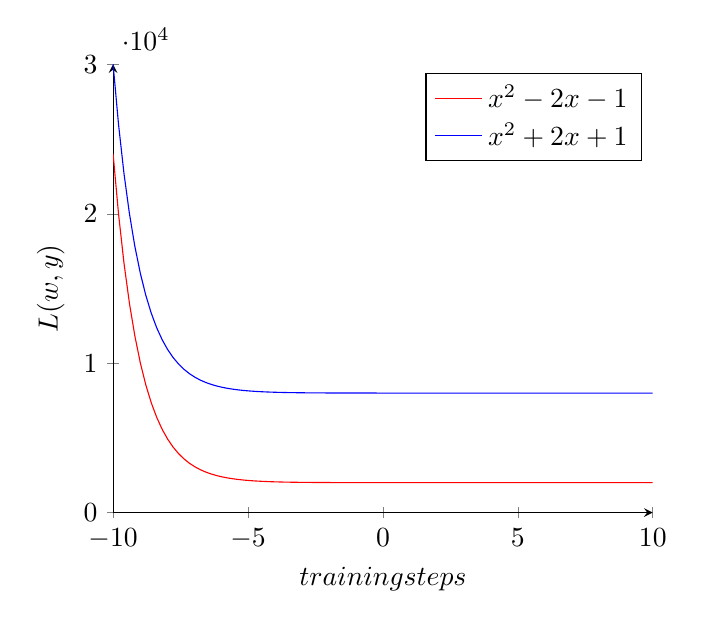
\begin{tikzpicture}
    \begin{axis}[
        axis lines = left,
        xlabel = $training steps$,
        ylabel = {$L(w,y)$},
        ymin=0,
    ]
    %Below the red parabola is defined
    \addplot [
        domain=-10:10, 
        samples=100, 
        color=red,
    ]
    {e^-x + 2000};
    \addlegendentry{$x^2 - 2x - 1$}
    %Here the blue parabloa is defined
    \addplot [
        domain=-10:10, 
        samples=100, 
        color=blue,
        ]
        {e^-x + 8000};
    \addlegendentry{$x^2 + 2x + 1$}
     
    \end{axis}
    \end{tikzpicture}
    \caption{irgend ein plot}
    \label{fig:ptl}
\end{figure}
% hier plot von train/val los

Grund dafür sind entweder zu wenige Trainingsdaten oder das Netz hat zu viele Neuronen, ist also 
überparametrisiert, und damit zu viele Freiheiten sich den Daten anzupassen. \ref{fig:overfit} 
\\
Hat das Modell zu wenige Parameter um die komplexität der Daten anzugleichen, Bsp, Gerade an Funktion 
höreren Grades, spricht man von Underfitting. \ref{fig:underfit}

% hier plots von linie durch datenpunkte


% Overfitting -> hohe varianz: varianz = train_err - test_error
% Underfitting -> hoher Bias: Bias = 


Um Overfitting zu vermeiden können entweder mehr Trainingsdaten verwendet werden. Stehen diese 
jedoch nicht zu verfügung, kann Regularisierung verwendet werden, eine Technik die neben der 
minimierung der Loss Funktion auch versucht die Gewichte auf einem kleinen Wert zu halten. 
Dafür wird der zu minimierenden Loss Function als weiterer 
Therm eine aufsummierung aller quadrieten Gewichte hinzugefügt. (\ref{eq:regularization}) 
\cite{geronHandsonMachineLearning2017}


\begin{equation}
    \label{eq:regularization}
    J(w) = E + \lambda \sum_{i} w_{i}^{2}
\end{equation}

% Early Stopping
Weitere Möglichkeiten sind Daten Augemntierung oder Drop Out, auf die 
in Abschnitt \ref{sec:deepl_cv} genauer eingegangen wird.



%########################################################################################
%##########################  SECTION: DEEP LEARNIN UNG COMPUTER VISION  #################
%########################################################################################
\section{Deep Learning und Computer Vision}\label{sec:deepl_cv}



Neben den in \ref{sec:nn} beschrieben sogenannten \textit{Feed Forward Netzen} 
gibt es eine vielzahl an Erweiterungen der Netzwerk Architektur, für unterschiedliche 
Anwendugsgebiete, die jedoch alle das beschriebene Grundprinzip verwenden.\\

Hat ein NN mehr als eine Hidden Schicht, spricht man von Deep Lerining.

Arten von NNs:
\begin{itemize}
    \item CNN: für bilder, durch faltung erkennt features und ist translatorisch invariant: \textbf{Image Classification}
    \item Recurrecnt Neural Networks/LSTM: durch feedback in network: für Audio und zeitl. anwendungen 
    \item Autoencoder, GANs, etc.
\end{itemize}

Computer Vision beschäftigt sich mit der Bild erkennung und Objekt Lokalisierung. 
Anwendungen sind gesichtserkennung oder Autonomes Fahren. 




%##########################  SUBSECTION:CNNs  ################################
\subsection{Convolutional Neural Networks}

Um Bilder /Inhalte mithilfe Neuronaler Netze zu erkennen, 
werden die einzelnen Pixelwerte der Bilder als Inputs verwendet 
und das auf dem Bild zu erkennende Objekt als output verwendet. Bilder 
werden als Matrizen der Form $height\times width \times color channels$ 
dargestellt.

Da dies für regulere/vollständig verbundene Neuronale Netze eine 
enorme Anzahl an Parametern und damit einhergenhender rechenkost 
bedeuten würde, werden hier CNNs verwendet, eine Architektur in 
der Paramer von verschiedenen Neuronen gemeinsam genutzt werden.

Hauptbestandteil von CNNs sind die \textit{Convolutional Layers}
welche die mathematische Faltungsoperation zwischen Input Bild 
und Filter/Kernel durchführen.

Die Filter meist der Form $3 \times 3$ oder $5 \times 5$ und mit der 
selben Tiefe wie der Input, werden während des \textit{Forward 
Pass/bropagation} zeilenweise über das Bild geschoben und an jeder Stelle 
das Kreuzprodukt berechnet. Jedes Ergebnis dieser berechnungen ergibt einen
Pixel Wert der nächsten Schicht auch Feature Map genannt. \ref{fig:cnn}

Ein weiterer bestandteil von CNNs sind die Pooling Layer, welche eine 
bestimmte Anzahl an Pixeln zB 3 x 3 zu einem Wert zusammenfassen wodurch 
sich die Parameter Anzahl des Bildes veringert. Das hat den Vorteil, dass 


\begin{figure}[htb]
    \centering
    \label{fig:lenet}
    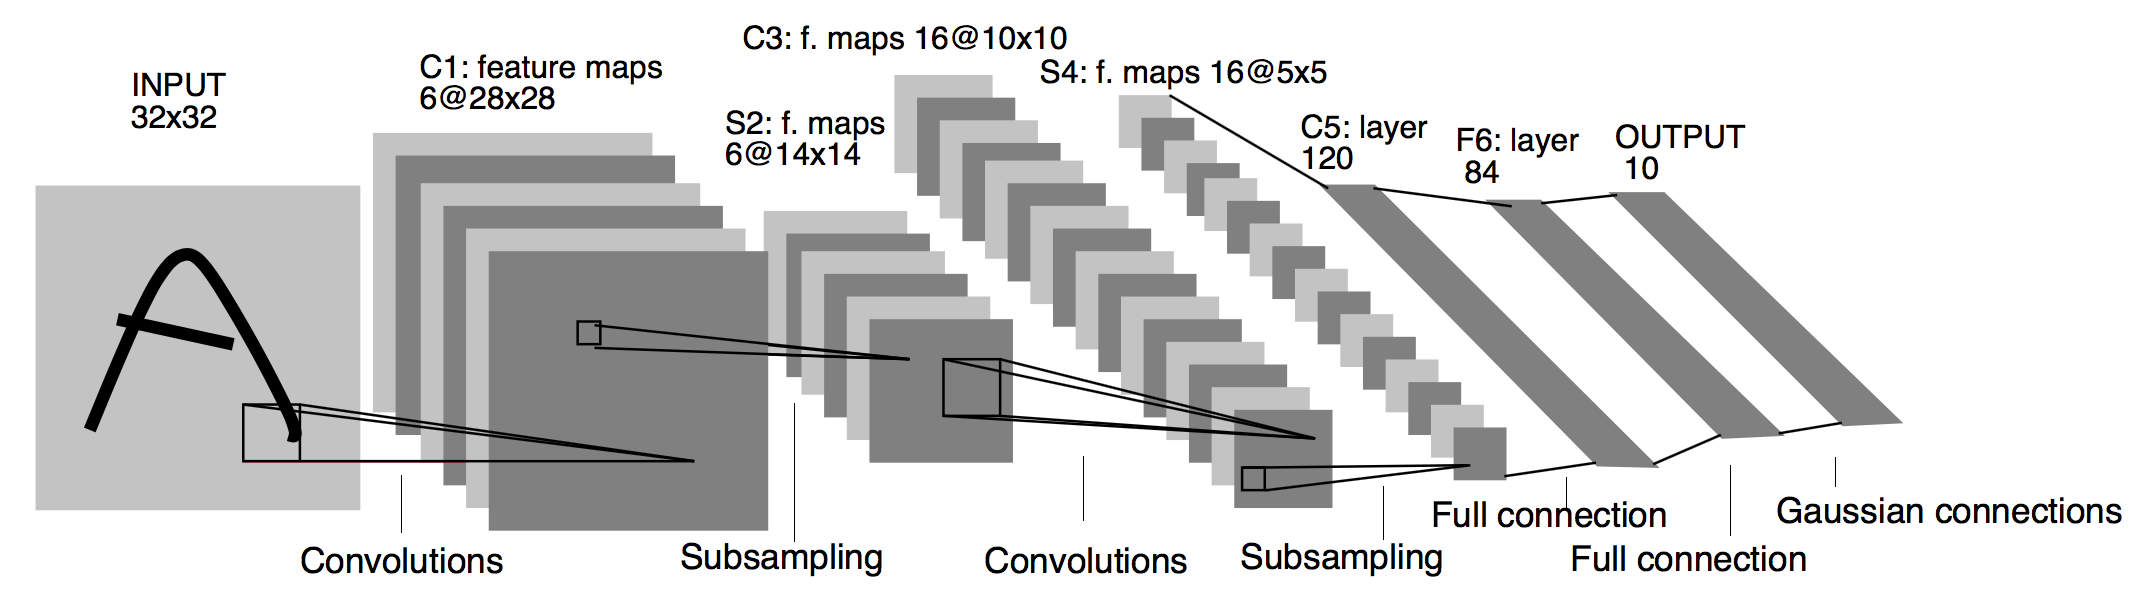
\includegraphics[width=0.8\textwidth]{Bilder/lenet.png}
    \caption{LeNet-5 cite lecun}
\end{figure}



Ziel dieser Operation ist es, dass die 
Filter Maps bestimmte Muster/features die zu einer bestimmten klasse 
gehren lernen. Mit diesen Filtern können dann unabhängig wo im Bild 
befindlich, die features wie zb horizontale/vertikale linien, Ecken 
oder Kreise gefunden werden. 
\\
Beispiel:
\begin{equation}
    \begin{pmatrix}
        1 & 0 & -1\\
        1 & 0 & -1\\
        1 & 0 & -1
    \end{pmatrix}
\end{equation}

erkennt vertikale Linien im Bild. 




Conv layer:\\
Faltung an cnn erklärt: input image als (h,w,c) tensor wird mit filter/kernel gefaltet. daraus erhält man feature map
zusammen mit pool layer:\\
pool layer erklärt\\

ergibt grundstruktur von cnn\\

weitere layer wie dropout\\

%##########################  SUBSECTION: TANSFER LEARINING  ################################
\subsection{Transfer Learining}

erklären, dass features von einfach bis immer komplexer werdende muster enthalten, die im bild zu finden sind.
\\
filter können zufällig initialisiert und gelernt werden, oder von vortrainierten netzen wieder verwendet
werden. (transfer learining oder fine tuning) da die deatures (besonders in den vorderen layern) immer ähnlich sind und das
neu lernen zeitaufwändig und oft sogar ungenauer ist.
\\
je nach ähnlichkeit des eig datensetz zu dem auf das netz urspr trainiert wurde:\\
scratch, fine tuning, feature extractor



%##########################  SUBSECTION: COMPETITIONS  ################################
\subsection{Competitions mit Imagenet und co + cnn winner}\label{subsec:comp}

zuerst competition erklären \\
dann chronologische gewinner netzt + besonderheit\\




%##########################  SUBSECTION: OBJEKT ERKENNUNG  ################################
\subsection{Objekt erkennung}\label{sec:objdet}


Unterschied deutlich machen: klassifikator kann nur ges bild auswertuen und wahscheinlichk angeben welche 
klasse darauf. keine lokalisierng und keine mult obj\\

3 Arten der Bilderkennung: Klassifizierung, Objekt Erkennung (für mult + box), Segmentation (jeden pixel)

dafür obj erkennung notw:\\

Single Shot Detectoren
\\

Two Stage Detectoren


%########################################################################################
%##########################  SECTION: HARDWARE  #################
%########################################################################################
\section{Hardware}\label{sec:hardware}
%noch eine section zu Hardware allg (cpu, gpu, tpu), Neural Compute Stick und AI on the egde


allg zu hardware für deeplearning. Das besser auf gpu als cpu. weitere: tpu, fpga, vpu, wie zb ncs2.

\subsection{Neural Compute Stick 2}

technischen spezifikationen





\subsection{AI on the edge}

was bedeutet dies. cloud unabhängig und ohne groß rechner. bsp anwendungen.

